


\tikzset{every picture/.style={line width=0.75pt}} %set default line width to 0.75pt        

\begin{tikzpicture}[x=0.75pt,y=0.75pt,yscale=-1,xscale=1]
%uncomment if require: \path (0,300); %set diagram left start at 0, and has height of 300

%Image [id:dp5400394261220618] 
\draw (345.17,143.14) node  {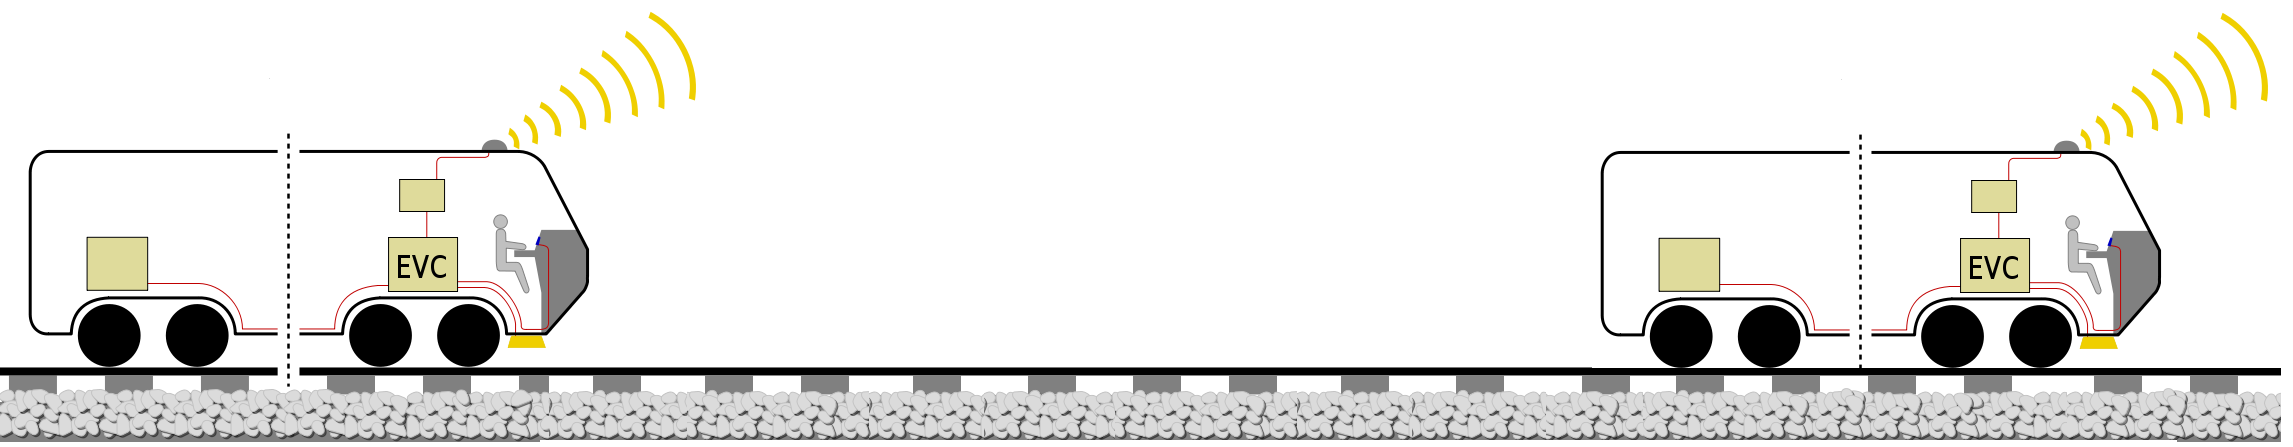
\includegraphics[width=451.25pt,height=87.97pt]{figure/ERTMS_Background.png}};
%Straight Lines [id:da10086853571322152] 
\draw [line width=1.5]    (200,217) -- (571.67,217) ;
\draw [shift={(575.67,217)}, rotate = 180] [fill={rgb, 255:red, 0; green, 0; blue, 0 }  ][line width=0.08]  [draw opacity=0] (11.61,-5.58) -- (0,0) -- (11.61,5.58) -- cycle    ;
\draw [shift={(200,217)}, rotate = 180] [color={rgb, 255:red, 0; green, 0; blue, 0 }  ][line width=1.5]    (0,6.71) -- (0,-6.71)   ;
%Straight Lines [id:da4246282135374029] 
\draw    (397,172) -- (463,172) ;
\draw [shift={(463,172)}, rotate = 180] [color={rgb, 255:red, 0; green, 0; blue, 0 }  ][line width=0.75]    (0,5.59) -- (0,-5.59)   ;
\draw [shift={(397,172)}, rotate = 180] [color={rgb, 255:red, 0; green, 0; blue, 0 }  ][line width=0.75]    (0,5.59) -- (0,-5.59)   ;
%Straight Lines [id:da8337786703307539] 
\draw [color={rgb, 255:red, 245; green, 166; blue, 35 }  ,draw opacity=1 ][line width=1.5]    (76.67,81.58) -- (153.17,82.58) ;
%Straight Lines [id:da7125538621487029] 
\draw  [dash pattern={on 4.5pt off 4.5pt}]  (397,60) -- (397.99,231.25) ;
\draw [shift={(398,233.25)}, rotate = 269.67] [color={rgb, 255:red, 0; green, 0; blue, 0 }  ][line width=0.75]    (10.93,-3.29) .. controls (6.95,-1.4) and (3.31,-0.3) .. (0,0) .. controls (3.31,0.3) and (6.95,1.4) .. (10.93,3.29)   ;
%Straight Lines [id:da421538735336056] 
\draw    (200,170.75) -- (397,172) ;
\draw [shift={(397,172)}, rotate = 180.36] [color={rgb, 255:red, 0; green, 0; blue, 0 }  ][line width=0.75]    (0,5.59) -- (0,-5.59)   ;
\draw [shift={(200,170.75)}, rotate = 180.36] [color={rgb, 255:red, 0; green, 0; blue, 0 }  ][line width=0.75]    (0,5.59) -- (0,-5.59)   ;
%Straight Lines [id:da6915654353430236] 
\draw [color={rgb, 255:red, 74; green, 144; blue, 226 }  ,draw opacity=1 ][line width=1.5]  [dash pattern={on 5.63pt off 4.5pt}]  (397,60) -- (73.67,60) ;
%Straight Lines [id:da3836173430907017] 
\draw [color={rgb, 255:red, 74; green, 144; blue, 226 }  ,draw opacity=1 ][line width=1.5]    (397,60) -- (528.33,60) ;
%Curve Lines [id:da5699852019251703] 
\draw [color={rgb, 255:red, 245; green, 166; blue, 35 }  ,draw opacity=1 ][line width=1.5]    (153.17,82.58) .. controls (212.33,-92.33) and (309.67,70) .. (397,60) ;
%Shape: Circle [id:dp11642118006555191] 
\draw  [fill={rgb, 255:red, 0; green, 0; blue, 0 }  ,fill opacity=1 ] (393.33,59.08) .. controls (393.33,56.55) and (395.39,54.5) .. (397.92,54.5) .. controls (400.45,54.5) and (402.5,56.55) .. (402.5,59.08) .. controls (402.5,61.61) and (400.45,63.67) .. (397.92,63.67) .. controls (395.39,63.67) and (393.33,61.61) .. (393.33,59.08) -- cycle ;
%Straight Lines [id:da5295755202589745] 
\draw [line width=1.5]    (75,106.33) -- (74.36,-6.33) ;
\draw [shift={(74.33,-10.33)}, rotate = 89.67] [fill={rgb, 255:red, 0; green, 0; blue, 0 }  ][line width=0.08]  [draw opacity=0] (11.61,-5.58) -- (0,0) -- (11.61,5.58) -- cycle    ;
\draw [shift={(75,106.33)}, rotate = 89.67] [color={rgb, 255:red, 0; green, 0; blue, 0 }  ][line width=1.5]    (0,6.71) -- (0,-6.71)   ;

% Text Node
\draw (96.17,54) node [anchor=north west][inner sep=0.75pt]  [font=\normalsize]  {$v_{F}$};
% Text Node
\draw (180.5,219) node [anchor=north west][inner sep=0.75pt]  [font=\normalsize]  {$s_{F}$};
% Text Node
\draw (411,145.5) node [anchor=north west][inner sep=0.75pt]  [font=\normalsize]  {$SM_{L4}$};
% Text Node
\draw (437.33,33.67) node [anchor=north west][inner sep=0.75pt]  [font=\normalsize]  {$v_{L}$};
% Text Node
\draw (62,124.5) node [anchor=north west][inner sep=0.75pt]  [color={rgb, 255:red, 245; green, 166; blue, 35 }  ,opacity=1 ] [align=left] {Follower};
% Text Node
\draw (470,123.5) node [anchor=north west][inner sep=0.75pt]  [color={rgb, 255:red, 74; green, 144; blue, 226 }  ,opacity=1 ] [align=left] {Leader};
% Text Node
\draw (383,232.5) node [anchor=north west][inner sep=0.75pt]   [align=left] {$s_{LoA}$};
% Text Node
\draw (206.67,3) node [anchor=north west][inner sep=0.75pt]    {$ \begin{array}{l}
{\gamma _{L4}}( t)\\
\end{array}$};
% Text Node
\draw (554.67,222.33) node [anchor=north west][inner sep=0.75pt]    {$s$};
% Text Node
\draw (54,-2.33) node [anchor=north west][inner sep=0.75pt]    {$v$};


\end{tikzpicture}